\newcommand{\substxy}[3]{\textcolor{#1}{[x\mapsto {#2}; y\mapsto {#3}]}}
\newcommand{\upperB}{\boxed{o}}
\newcommand{\lowerB}{\boxed{u}}

\begin{frame}[fragile]
    \frametitle{Preliminaries}

\begin{definition}[Substitution] 
    A substitution $\sigma: \Code{Var} \rightharpoonup \Code{Value}$ is a partial function (mapping) from variables to resources.
\end{definition}

\begin{definition}[Piontwise Union] $m_1 \times m_2 \doteq \{ \sigma_1 \cup \sigma_2 ~|~ \sigma_1 \in m_1 \land \sigma_2 \in m_2 \}$.
\end{definition}
    
\end{frame}

\begin{frame}[fragile]
    \frametitle{Choice Algebra}

\begin{definition}[Choice Algebra] A choice algebra is a tuple $(M, \mathbf{0}, \mathbf{1}, +, \times)$ where:
    \begin{itemize}
        \item A resource $m$ is a set of substitutions: $\mathcal{P}(\Code{Var} \rightharpoonup \Code{Value})$.
        \item $M$ is the set of resources.
        \item $\mathbf{0}$ is $\emptyset$.
        \item $\mathbf{1}$ is $\{\emptyset\}$.
        \item $+$ is the union operation; $\wfvdash m_1 + m_2$ iff $\Code{Dom}(m_1) = \Code{Dom}(m_2)$.
        \item $\times$ is the pointwise union operation; $\wfvdash m_1 \times m_2$ iff
        \begin{align*}
            &\Code{Dom}(m_1) \cap \Code{Dom}(m_2) = \emptyset
        \end{align*} 
        % \begin{align*}
        %     &\forall \sigma_1 \in m_1, \forall \sigma_2 \in m_2. 
        %     \\&\qquad \forall x. x \in \Code{Dom}(\sigma_1) \land x \in \Code{Dom}(\sigma_2) \implies \sigma_1(x) = \sigma_2(x)
        % \end{align*}
    \end{itemize}
\end{definition}
    
\end{frame}

\begin{frame}[fragile]
    \frametitle{Choice Algebra: Problem}

We try to build a unified logic over this algebra.

\textbf{Problem:} If we want to enable both the over- and under-approximation reasoning, how can we define Kripke's Monotonicity?

\begin{lemma}[Kripke's Monotonicity]
    $m \leq m'$ and $m \models\phi$ implies $m' \models\phi$.
\end{lemma}

\textbf{Problem:} $\phi$ can be an overapproximated or underapproximated proposition. The direction of the partial order should be reversed. More complicated, $\Code{Over} \land \Code{Under}$.
    
\end{frame}

\begin{frame}[fragile]
    \frametitle{Choice Algebra: Partial Order}

\textbf{Intuition:} Assume $a + b = c$. It is hard to decide if $a \leq c$, since we must consider both overapproximation and underapproximation.

\textbf{Intuition:} If $a \times b = c$, we always have $a \models\phi$ implies $c \models\phi$.

\begin{definition}[Partial Order]
    \[
    m_1 \leq m_2 \doteq
    \begin{cases}
        \exists m_3.\ m_1 \times m_3 = m_2 & \text{when } \Code{Dom}(m_1) \subseteq \Code{Dom}(m_2) \\
        \text{undefined} & \text{otherwise}
    \end{cases}
    \]
\end{definition}

\begin{definition}[Projection]
    \begin{align*}
    &\Code{Proj}(X, \sigma) \doteq
        \begin{cases}
            \bigcup_{x \in X} [x\mapsto \sigma(x)] & \text{when } X \subseteq \Code{Dom}(\sigma) \\
            \text{undefined} & \text{otherwise}
        \end{cases}
    \\&\Code{Proj}(X, m) \doteq
    \begin{cases}
        \bigcup_{\sigma \in m} \{ \Code{Proj}(X, \sigma) \} & \text{when } X \subseteq \Code{Dom}(m_2) \\
        \text{undefined} & \text{otherwise}
    \end{cases}
    \end{align*}
\end{definition}

\end{frame}

\begin{frame}[fragile]
    \frametitle{Basic Choice Logic}

\begin{definition}[Atomic Propositions] Atomic proposition $P: M \sarr \Bool$ is a predicate over resources.
\end{definition}

\begin{definition}[Basic Choice Logic] Basic choice logic has no approximation; everything needs to be precise.
\end{definition}
\begin{itemize}
    \item $m \models\phi * \psi$ iff $\exists m_1, m_2.\ m_1 \times m_2 \leq m \text{ and } m_1 \models\phi \text{ and } m_2 \models\psi$.
    \item $m \models\phi \wand \psi$ iff $\forall m'. m' \models\phi  \implies m' \times m \models\psi$.
    \item $m \models\phi \oplus \psi$ iff $\exists m_1, m_2.\ m_1 + m_2 \leq m \text{ and } m_1 \models\phi \text{ and } m_2 \models\psi$.
    \item $m \models P$ iff $\{\sigma ~|~ \Code{Dom}(\sigma) = \Code{FV}(\phi) \land \sigma(P)\}\leq m$.
    \item $m \models\true$ always; $m \models\false$ \textcolor{red}{iff $m = \mathbf{0}$}.
    \item $m \models\phi \land \psi$ iff $m \models\phi$ and $m \models\psi$.
    \item $m \models\phi \implies \psi$ iff $m \models\phi$ implies $m \models\psi$.
    \item $m \models\phi \lor \psi$ iff $m \models\phi$ or $m \models\psi$.
    \item $m \models\forall x. \phi$ iff for all $v$, $m \models\phi[x\mapsto v]$.
    \item $m \models\exists x. \phi$ iff there exists $v$ such that $m \models\phi[x\mapsto v]$.
\end{itemize}

\end{frame}

\begin{frame}[fragile]
    \frametitle{Basic Choice Logic}

\begin{example} Consider variable $x$ of type $\Nat$.
    \begin{itemize}
        \item $\{[x\mapsto 0], [x\mapsto 1]\} \models x < 2$.
        \item $\{[x\mapsto 0], [x\mapsto 1], [x\mapsto 2]\} \not\models x < 2$.
        \item $\{[x\mapsto 0]\} \not\models x < 2$.
        \item $\{\substxy{blue}{0}{1}, \substxy{orange}{1}{0}\} \models x < 2$.
    \end{itemize}
\end{example}

\end{frame}

\begin{frame}[fragile]
    \frametitle{Basic Choice Logic: Dependency}

\begin{example} Consider variables $x$ and $y$ of type $\Nat$.
    \begin{itemize}
        \item $\{\substxy{blue}{0}{1}, \substxy{orange}{1}{0}\} \models x < 2 \land y < 2$.
        \item $\{\substxy{blue}{0}{1}, \substxy{red}{0}{0}, \substxy{orange}{1}{0}\} \models x < 2 \land y < 2$.
        \item $\{\substxy{blue}{0}{1}, \substxy{red}{0}{0}, \substxy{orange}{1}{0}, \substxy{DeepGreen}{1}{1}\} \models x < 2 \land y < 2$.
        \item $\{\substxy{blue}{0}{1}, \substxy{red}{0}{0}, \substxy{orange}{1}{0}, \substxy{DeepGreen}{1}{1}\} \models x < 2 * y < 2$.
    \end{itemize}
\end{example}

\textbf{Intuition:} Even if the logic is precise for a single variable, there is still imprecision caused by the dependency of variables.

\end{frame}

\begin{frame}[fragile]
    \frametitle{Basic Choice Logic: Sum}

\begin{example} Consider variables $x$ and $y$ of type $\Nat$.
    \begin{itemize}
        \item $\{[x\mapsto 1]\} \models x = 1 \lor x = 2$.
        \item $\{[x\mapsto 2]\} \models x = 1 \lor x = 2$.
        \item $\{[x\mapsto 1], [x\mapsto 2]\} \not\models x = 1 \lor x = 2$.
        \item $\emptyset \not\models x = 1 \lor x = 2$.
        \item There is no resource that can model $x = 1 \land x = 2$.
        \item The formula $x = 1 * x = 2$ is not well-formed.
        \item $\{[x\mapsto 1], [x\mapsto 2]\} \models x = 1 \oplus x = 2$.
        \item $\{\substxy{blue}{1}{2}, \substxy{orange}{2}{1}\} \models x = 1 \oplus x = 2$.  
    \end{itemize}
\end{example}

\textbf{Intuition:} The $\oplus$ operator means the choices can be divided into two groups.

\end{frame}

\begin{frame}[fragile]
    \frametitle{Basic Choice Logic: Monotonicity}

\begin{lemma}[Kripke's Monotonicity]
        $m \leq m'$ and $m \models\phi$ implies $m' \models\phi$.
\end{lemma}

\end{frame}

\begin{frame}[fragile]
    \frametitle{Pure Propositions}

Assume we have an expressive enough atomic proposition $P: M \sarr \Bool$:
\begin{align*}
P \doteq \Code{Atom} ~|~ \Code{Dom}(X) ~|~ P \cap P ~|~ P \cup P ~|~ P \setminus P ~|~ P \times P
\end{align*}
where
\begin{itemize}
    \item $\Code{Atom}$ is an atomic proposition, e.g., $x < 2$.
    \item $\Code{Dom}(X)$ make sure all substitutions has the same domain as $X$.
    \item $P \cap Q$ is the intersection of $P$ and $Q$.
    \item $P \cup Q$ is the union of $P$ and $Q$.
    \item $P \setminus Q$ is the difference of $P$ and $Q$.
    \item $P \times Q$ is the pointwise union of $P$ and $Q$.
\end{itemize}

\end{frame}

\begin{frame}[fragile]
    \frametitle{Choice Logic with Approximation}

\begin{definition}[Choice Logic with Approximation] We consider two new modalities, $\upperB$ and $\lowerB$.
    \begin{itemize}
        \item $m \models\upperB\phi$ iff $\exists m_1, m'.\ m + m_1 = m' \text{ and } m' \models\phi$.
        \item $m \models\lowerB\phi$ iff $\exists m_1, m'.\ m' + m_1 = m  \text{ and } m' \models\phi$.
    \end{itemize}
\end{definition}

\textbf{Intuition:} They work like the upper and lower bounds of a resource.

\begin{example}
    \begin{itemize}
        \item $\{[x\mapsto 0]\} \models\upperB(x < 2)$.
        \item $\{[x\mapsto 0], [x\mapsto 1], [x\mapsto 2]\} \models\lowerB(x < 2)$.
        \item $\{[x\mapsto 0], [x\mapsto 1], [x\mapsto 2]\} \models\upperB(x < 4) \land \lowerB(x < 2)$.
    \end{itemize}
\end{example}

\end{frame}

\begin{frame}[fragile]
    \frametitle{Denotation}

\begin{definition}[Denotation] We define $\denot{\phi}$ as the set of resources that model $\phi$ (we assume all resource has the same domain with the properties).
\begin{itemize}
    \item $\denot{\upperB\phi} = \bigcup_{m \in \denot{\phi}} \{ m' ~|~ m' \subseteq m \}$
    \item $\denot{\lowerB\phi} = \bigcup_{m \in \denot{\phi}} \{ m' ~|~ m \subseteq m' \}$
    \item $\denot{\phi_1 \land \phi_2} = \denot{\phi_1} \cap \denot{\phi_2}$, $\denot{\phi_1 \lor \phi_2} = \denot{\phi_1} \cup \denot{\phi_2}$
    \item $\denot{\phi_1 \implies \phi_2} = \denot{\phi_1} \subseteq \denot{\phi_2}$
    \item $\denot{\true} = M$;  $\denot{\false} = \{\mathbf{0}\}$
    \item $\denot{\phi_1 * \phi_2} = \{ m_1 \times m_2 ~|~ m_1 \in \denot{\phi_1} \land m_2 \in \denot{\phi_2} \}$
    \item $\denot{\phi_1 \oplus \phi_2} = \{ m_1 + m_2 ~|~ m_1 \in \denot{\phi_1} \land m_2 \in \denot{\phi_2} \}$
    \item $\denot{\phi_1 \wand \phi_2} = \{ m ~|~ \forall m_1 \in \denot{\phi_1}.\ m_1 \times m \in \denot{\phi_2} \}$
\end{itemize}
\end{definition}

\begin{lemma}[Idempotency]
    $\upperB\phi \vdash \upperB\upperB\phi$ and $\lowerB\phi \vdash \lowerB\lowerB\phi$.
\end{lemma}

\end{frame}

\begin{frame}[fragile]
    \frametitle{Properties of Approximation}

\begin{definition}[Approximation Normal Form (AppNF)] The $\upperB$ and $\lowerB$ modalities appear only before atomic propositions.
\end{definition}

\textbf{Question:} Can all formulas be converted to AppNF?

% \begin{definition}[Polarity] A property $p$ is overapproximated iff $\forall m, m'.\ m \subseteq m' \land m' \in \denot{p} \implies m \in \denot{p}$. A property $p$ is overapproximated iff $\forall m, m'.\ m \subseteq m' \land m' \in \denot{p} \implies m \in \denot{p}$.
% \end{definition}

Let $p$ and $q$ be modality-free propositions (constructed from $P$, $\land$, $\lor$, $\implies$, $\true$, $\false$).

\begin{lemma}[Overapproximation] Consider the modality-free propositions $p$ and $q$.
\begin{itemize}
    \item $\upperB p \land \upperB q \dashv\vdash \upperB(p \cap q)$, thus $\upperB(\upperB p \land \upperB q) \dashv\vdash \upperB(p \cap q)$. 
    \item $\upperB(\upperB p \lor \upperB q) \dashv\vdash \upperB p \lor \upperB q$.
    \item $\upperB p \implies \upperB q \dashv\vdash \upperB(p \implies q)$, similar to $\land$.
    \item $\upperB \true \dashv\vdash \true$; $\upperB \false \dashv\vdash \false$.
    % \item $\lowerB p \land \lowerB q \dashv\vdash \lowerB(p \land q)$ 
\end{itemize}
\end{lemma}

\end{frame}

\begin{frame}[fragile]
    \frametitle{Properties of Approximation}

\begin{definition}[All] We introduce a new atomic predicate $\Code{All}$ parameterized by a set of variables: $m \models \Code{All}(X) \doteq m = \{\sigma ~|~ \Code{Dom}(\sigma) = X\}$.
\end{definition}

\begin{lemma}[Cancel Out]
    $\upperB\lowerB p \dashv\vdash \upperB\Code{All}(\Code{FV}(p))$ and $ \lowerB\upperB p \dashv\vdash \true$.
\end{lemma}
\begin{proof}
\begin{itemize}
    \item For $m \models \upperB\lowerB p$, $\Code{FV}(p) \subseteq \Code{Dom}(m)$. Thus $m \subseteq \denot{\Code{All}(\Code{FV}(p))}$.
    \item For $m \models \upperB \Code{All}(\Code{FV}(p))$, there exists $m' \doteq \denot{\Code{All}(\Code{FV}(p))}$ such that $m \subseteq m'$ and $\denot{p} \subseteq m'$.
    \item Note that for all $m$, $\textbf{0} \subseteq m$ and $\textbf{0} \subseteq \denot{p}$.
\end{itemize}
\end{proof}

\end{frame}


\begin{frame}[fragile]
    \frametitle{Properties of Approximation}

\begin{figure}[h!]
    \centering
    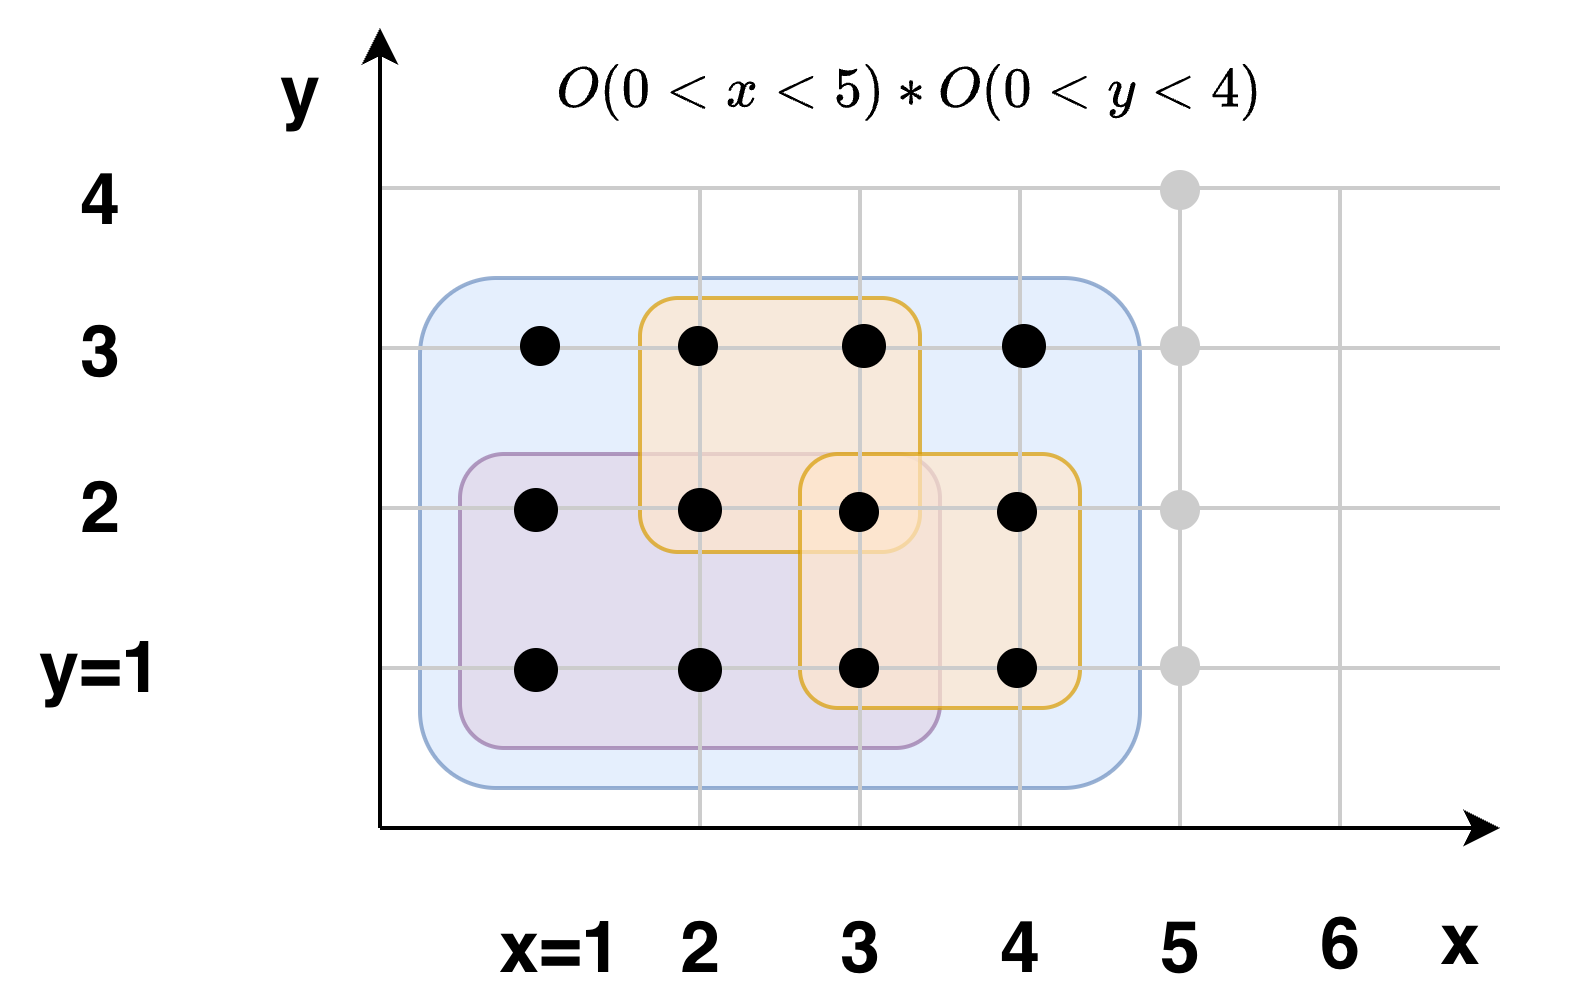
\includegraphics[width=0.8\textwidth]{figures/Ex4.drawio.png}
\end{figure}

\begin{lemma}[Merge Rule] $\upperB(\upperB p * \upperB q) \dashv\vdash \upperB(p * q) \dashv\vdash \upperB(p\land q)$.
\end{lemma}

\end{frame}

\begin{frame}[fragile]
    \frametitle{Properties of Approximation}

\begin{lemma}[Over Cancels $\oplus$] $\upperB p \oplus \upperB q \dashv\vdash \upperB (p \lor q)$.
\end{lemma}
\begin{proof}
    \begin{itemize}
        \item \textbf{Forward:} $m \models \upperB p \oplus \upperB q$ means there exist $m_1, m_2$ such that $m = m_1 + m_2$, $m_1 \models \upperB p$, and $m_2 \models \upperB q$. Thus $m_1 \in \denot{p}$ and $m_2 \in \denot{q}$, so $m = m_1 + m_2 \in \denot{p} \cup \denot{q} = \denot{p \lor q}$.
        \item \textbf{Backward:} $m \models \upperB p \oplus \upperB q$ means $m \subseteq \denot{p} \cup \denot{q}$. Thus $m = (m \cap \denot{p}) + (m \setminus \denot{p})$.
    \end{itemize}
\end{proof}

\begin{lemma}[Over Cancels $\oplus$] $\upperB(\upperB p \oplus \upperB q) \dashv\vdash \upperB (p \lor q)$.
\end{lemma}

\end{frame}

\begin{frame}[fragile]
    \frametitle{Properties of Approximation}

\begin{lemma}[Underapproximation] Consider the modality-free propositions $p$ and $q$.
\begin{itemize}
    \item $\lowerB p \land \lowerB q \dashv\vdash \lowerB(p \lor q)$.
    \item $\lowerB(\lowerB p \lor \lowerB q) \dashv\vdash \lowerB p \lor \lowerB q$.
    \item $\lowerB p \implies \lowerB q \dashv\vdash \lowerB(q \implies p)$, similar to $\land$.
    \item $\lowerB \true \dashv\vdash \true$; $\lowerB \false \dashv\vdash \true$.
\end{itemize}
\end{lemma}

\end{frame}

\begin{frame}[fragile]
    \frametitle{Properties of Approximation}

\begin{lemma}[Under Cancels $*$] $\lowerB(\lowerB p * \lowerB q) \dashv\vdash \lowerB (p * q)$; note that $\lowerB (p * q)$ is not equal to $\lowerB (p \land q)$.
\end{lemma}

\begin{lemma}[Merge Rule] $\lowerB p \oplus \lowerB q \dashv\vdash \lowerB (p \lor q)$.
\end{lemma}

\end{frame}

\begin{frame}[fragile]
    \frametitle{Properties of Approximation}

Consider the mixed case:

\begin{lemma}[Mixed Conjunction] $\upperB(\lowerB p \land \upperB q) \dashv\vdash \upperB q \land (p \impl q)$ and $\lowerB(\lowerB p \land \upperB q) \dashv\vdash (p \impl q) \impl \lowerB p$.
\end{lemma}

\end{frame}

\begin{frame}[fragile]
    \frametitle{Properties of Approximation}

Consider the mixed case:

\begin{lemma}[Mixed Disjunction] $\upperB(\lowerB p \lor \upperB q) \dashv\vdash \true$ and $\lowerB(\lowerB p \lor \upperB q) \dashv\vdash \true$.
\end{lemma}
\begin{proof}
    \begin{itemize}
        \item For all possible $m$, we have $m \subseteq \denot{p} \cup m$, and $\denot{p} \cup m \models \lowerB p$, thus $m \models \upperB(\lowerB p \lor \upperB q)$.
        \item For all possible $m$, we have $\denot{q} \cap m \subseteq m$, and $\denot{q} \cap m \models \upperB q$, thus $m \models \lowerB(\lowerB p \lor \upperB q)$.
    \end{itemize}
\end{proof}

\end{frame}

\begin{frame}[fragile]
    \frametitle{Properties of Approximation}

\begin{lemma}[Mixed $*$] $\upperB(\lowerB p * \upperB q) \dashv\vdash \upperB (\Code{All}(\Code{Dom}(p)) * q)$ and $\lowerB(\lowerB p * \upperB q) \dashv\vdash \true$.
\end{lemma}
\begin{proof} 
    \begin{itemize}
        \item \textbf{1. Forward:} $m\models \upperB(\lowerB p * \upperB q)$ means there exist $m_1, m_2$ such that $m \subseteq m_1 \times m_2$ and $m_1 \models \lowerB p$ and $m_2 \models \upperB q$. Thus $m_2 \subseteq \denot{q}$. It is easy to see that $m \subseteq \denot{\Code{All}(\Code{Dom}(p))} \times \denot{q}$. 
        \item \textbf{1. Backward:} $m \models \upperB (\Code{All}(\Code{Dom}(p)) * q)$ means there exist $m_1, m_2$ with $m_1 \in \denot{\Code{All}(\Code{Dom}(p))}$ and $m_2 \in \denot{q}$ such that $m \subseteq m_1 \times m_2$. It is easy to see that $m_1 \models \lowerB p$ and $m_2 \models \upperB q$.
        \item \textbf{2.} Note that $\textbf{0} = \denot{p} \times \textbf{0}$ and $\textbf{0} \models \upperB q$, thus $\textbf{0} \models \lowerB p * \upperB q$. 
    \end{itemize}
\end{proof}
\end{frame}

\begin{frame}[fragile]
    \frametitle{Properties of Approximation}

\begin{lemma}[Mixed $\oplus$] $\upperB(\lowerB p \oplus \upperB q) \dashv\vdash \upperB \Code{All}(\Code{Dom}(p))$ and $\lowerB(\lowerB p \oplus \upperB q) \dashv\vdash \lowerB p$.
\end{lemma}
\begin{proof} 
    \begin{itemize}
        \item \textbf{1.} For all $m$ whose domain is $\Code{Dom}(p)$, we have $m \subseteq (m \cup \denot{p}) + \textbf{0}$.
        \item \textbf{2. Forward:} $m\models\lowerB(\lowerB p \oplus \upperB q)$ means there exist $m_1, m_2$ such that $m_1 + m_2 \subseteq m$, $\denot{p} \subseteq m_1$, and $m_2 \subseteq \denot{q}$. We have $m_1 \subseteq m$.
        \item \textbf{1. Backward:} When $m\models \lowerB p$, we can choose $m + \textbf{0} \subseteq m$.
    \end{itemize}
    Note that $\lowerB p \oplus \upperB q \dashv\vdash \lowerB p \oplus \false \dashv\vdash \lowerB p$.
\end{proof}

\end{frame}

\begin{frame}[fragile]
    \frametitle{Simplified Choice Logic with Approximation}

\textbf{Idea:} We have proved that all formulas can be converted to AppNF, as long as our atomic propositions include $\Code{All}$.

\begin{definition}[Simplified Choice Logic with Approximation] The syntax is:
\begin{align*}
    \textbf{Variables} \quad x, y, z  \\
    \textbf{Variable Sets} \quad X, Y, Z \\
    \textbf{Constants} \quad c ::= & () ~|~ \mathbb{B} ~|~ \mathbb{Z} ~|~ ...  \\
    \textbf{Atomic Propositions} \quad P ::= & \Code{All}(X) ~|~ ...  \\
    \textbf{Propositions} \quad \phi ::= & \upperB P ~|~ \lowerB P ~|~ P ~|~ \phi \land \phi ~|~ \phi \lor \phi ~|~ \phi \implies \phi\\
    & ~|~ \forall x. \phi ~|~ \exists x. \phi ~|~ \true ~|~ \false \\
    & ~|~ \phi * \phi ~|~ \phi \oplus \phi ~|~ \phi \wand \phi
\end{align*}
\end{definition}

\end{frame}